\documentclass[smaller,aspectratio=1610,handout]{beamer}
\usepackage[utf8]{inputenc}
\usepackage[czech]{babel}
\usepackage[T1]{fontenc}
\usepackage{lmodern}
\usepackage{krskasugar}
\usepackage{fkssugar}
\usepackage{booktabs}
\usepackage{subcaption}

%\usepackage[
%	backend=biber,        % if we want unicode and many other features (biber is already by default)
%	style=iso-numeric,    % iso-numeric for numeric citation method
%	sorting=nty,          % for alphabetic sorting by author
%	sortcites=true
%]{biblatex}


\author[A. Krška]{Adam Krška}
\title[Stanovení parametru termočlánku]{Stanovení parametru termočlánku pomocí
metody nejmenších čtverců}
\subtitle{Seminární práce}
\institute[GSS Mikulov]{Gymnázium a střední odborná škola Mikulov}
\date{}

\usetheme{Frankfurt}
\usefonttheme{professionalfonts}
\usecolortheme{rose}
\useinnertheme{circles}
%\setbeamercovered{transparent} 
%\setbeamertemplate{navigation symbols}{} 

\graphicspath{{./graf/}{./figures/}}
%\addbibresource{sources.bib}

\newcommand\avg[1]{\mkern 1.5mu\overline{\mkern-1.5mu#1\mkern-1.5mu}\mkern 1.5mu}
\newcommand\sumi{\sum_{i=1}^n}

\begin{document}
\frame[plain]{\titlepage}

\begin{frame}{Obsah}
	\tableofcontents
\end{frame}

\section{Úvod}
\begin{frame}
	\frametitle{Úvod}
	\framesubtitle{Cíl experimentu}
	\begin{itemize}
		\item vlastnoruční sestavení termočlánku typu~T
		\item experimentální měření dat termočlánku
		\item výpočet parametru termočlánku pomocí metody nejmenších čtverců
	\end{itemize}	
\end{frame}


\begin{frame}
	\frametitle{Úvod}
	\framesubtitle{Zdroje}
	\begin{itemize}
		\item využito 11 zdrojů
		\item internetové zdroje, vysokoškolské skripta, bakalářské práce\dots
	\end{itemize}
\end{frame}

%\section{Současný stav problematiky} \subsection{Proložení dat funkcí}
%
%\begin{frame}
%	\frametitle{Proložení dat funkcí}
%	\framesubtitle{Aproximace a interpolace}
%	
%	\begin{block}{Interpolace}
%		Spojení všech bodů spojitou křivkou.	
%	\end{block}
%
%	\begin{block}{Aproximace}
%		Hledání předpisu funkce vhodně vyjadřující datové body.	
%	\end{block}
%\end{frame}
%
%\begin{frame}
%	\frametitle{Proložení dat funkcí}
%	\framesubtitle{Metoda nejmenších čtverců}
%	\begin{itemize}
%		\item metoda pro nalezení parametrů předpisu funkce
%		\item minimalizace druhých mocnin odchylek dat a funkce 
%	\end{itemize}
%	\begin{block}{Hledání minima funkce}
%	\vspace*{-0.2\baselineskip}\setlength\belowdisplayshortskip{0pt}
%	\eq{S=\sumi\(y_i-f(x_i)\)^2}
%	\end{block}
%
%	\begin{itemize}
%		\item metody řešení
%			\begin{itemize}
%				\item iterativně
%				\item analyticky
%			\end{itemize}
%	\end{itemize}
%\end{frame}
%
%\begin{frame}
%	\frametitle{Proložení dat funkcí}
%	\framesubtitle{Lineární regrese}
%	\begin{itemize}
%		\item speciální případ prokládání dat
%		\item aproximace lineární funkcí
%		\item analytické řešení
%	\end{itemize}
%\end{frame}
%
%\subsection{Termoelektrický jev}
%
%\begin{frame}
%	\frametitle{Termoelektrický jev}
%	\begin{itemize}
%		\item souhrnný název pro více efektů
%			\begin{itemize}
%				\item Seebeckův efekt
%				\item Peltierův efekt
%				\item Thomsonův efekt
%				\item Benedickův efekt
%			\end{itemize}
%		\item popis souvislosti elektrického napětí a rozdílu teplot
%	\end{itemize}
%\end{frame}
%
%\begin{frame}
%	\frametitle{Termoelektrický jev}
%	\framesubtitle{Termočlánky}
%	\begin{columns}
%		\begin{column}{0.6\textwidth}
%			\begin{itemize}
%				\item spojení dvou druhů kovů
%				\item rozdíl teplot spojů vede k vytvoření napětí
%				\item různé kombinace kovů -- různé vlastnosti
%				\item standard IEC 584
%			\end{itemize}
%		\end{column}
%		\begin{column}{0.4\textwidth}
%			\fullfig[width=0.9\linewidth]{termoclanek}
%		\end{column}
%	\end{columns}
%\end{frame}


\section{Metodika}
\begin{frame}
	\frametitle{Metodika}
	\begin{columns}
		\begin{column}{0.5\textwidth}
			\begin{enumerate}
				\item sestavení vlastního termočlánku z mědi a~konstantanu
				\item změření termoelektrického jevu
					\begin{itemize}
						\item ohřívání a ochlazování konců termočlánku
					\end{itemize}
				\item stanovení parametru $\alpha$ pro tento termočlánek
			\end{enumerate}
		\end{column}
		\begin{column}{0.5\textwidth}
			\fullfig[width=0.9\linewidth]{schema_stavba}
		\end{column}
	\end{columns}
\end{frame}

\begin{frame}
	\begin{figure}[htpb]
		\hfill
		\centering
		\begin{subfigure}{0.48\textwidth}
			\centering
			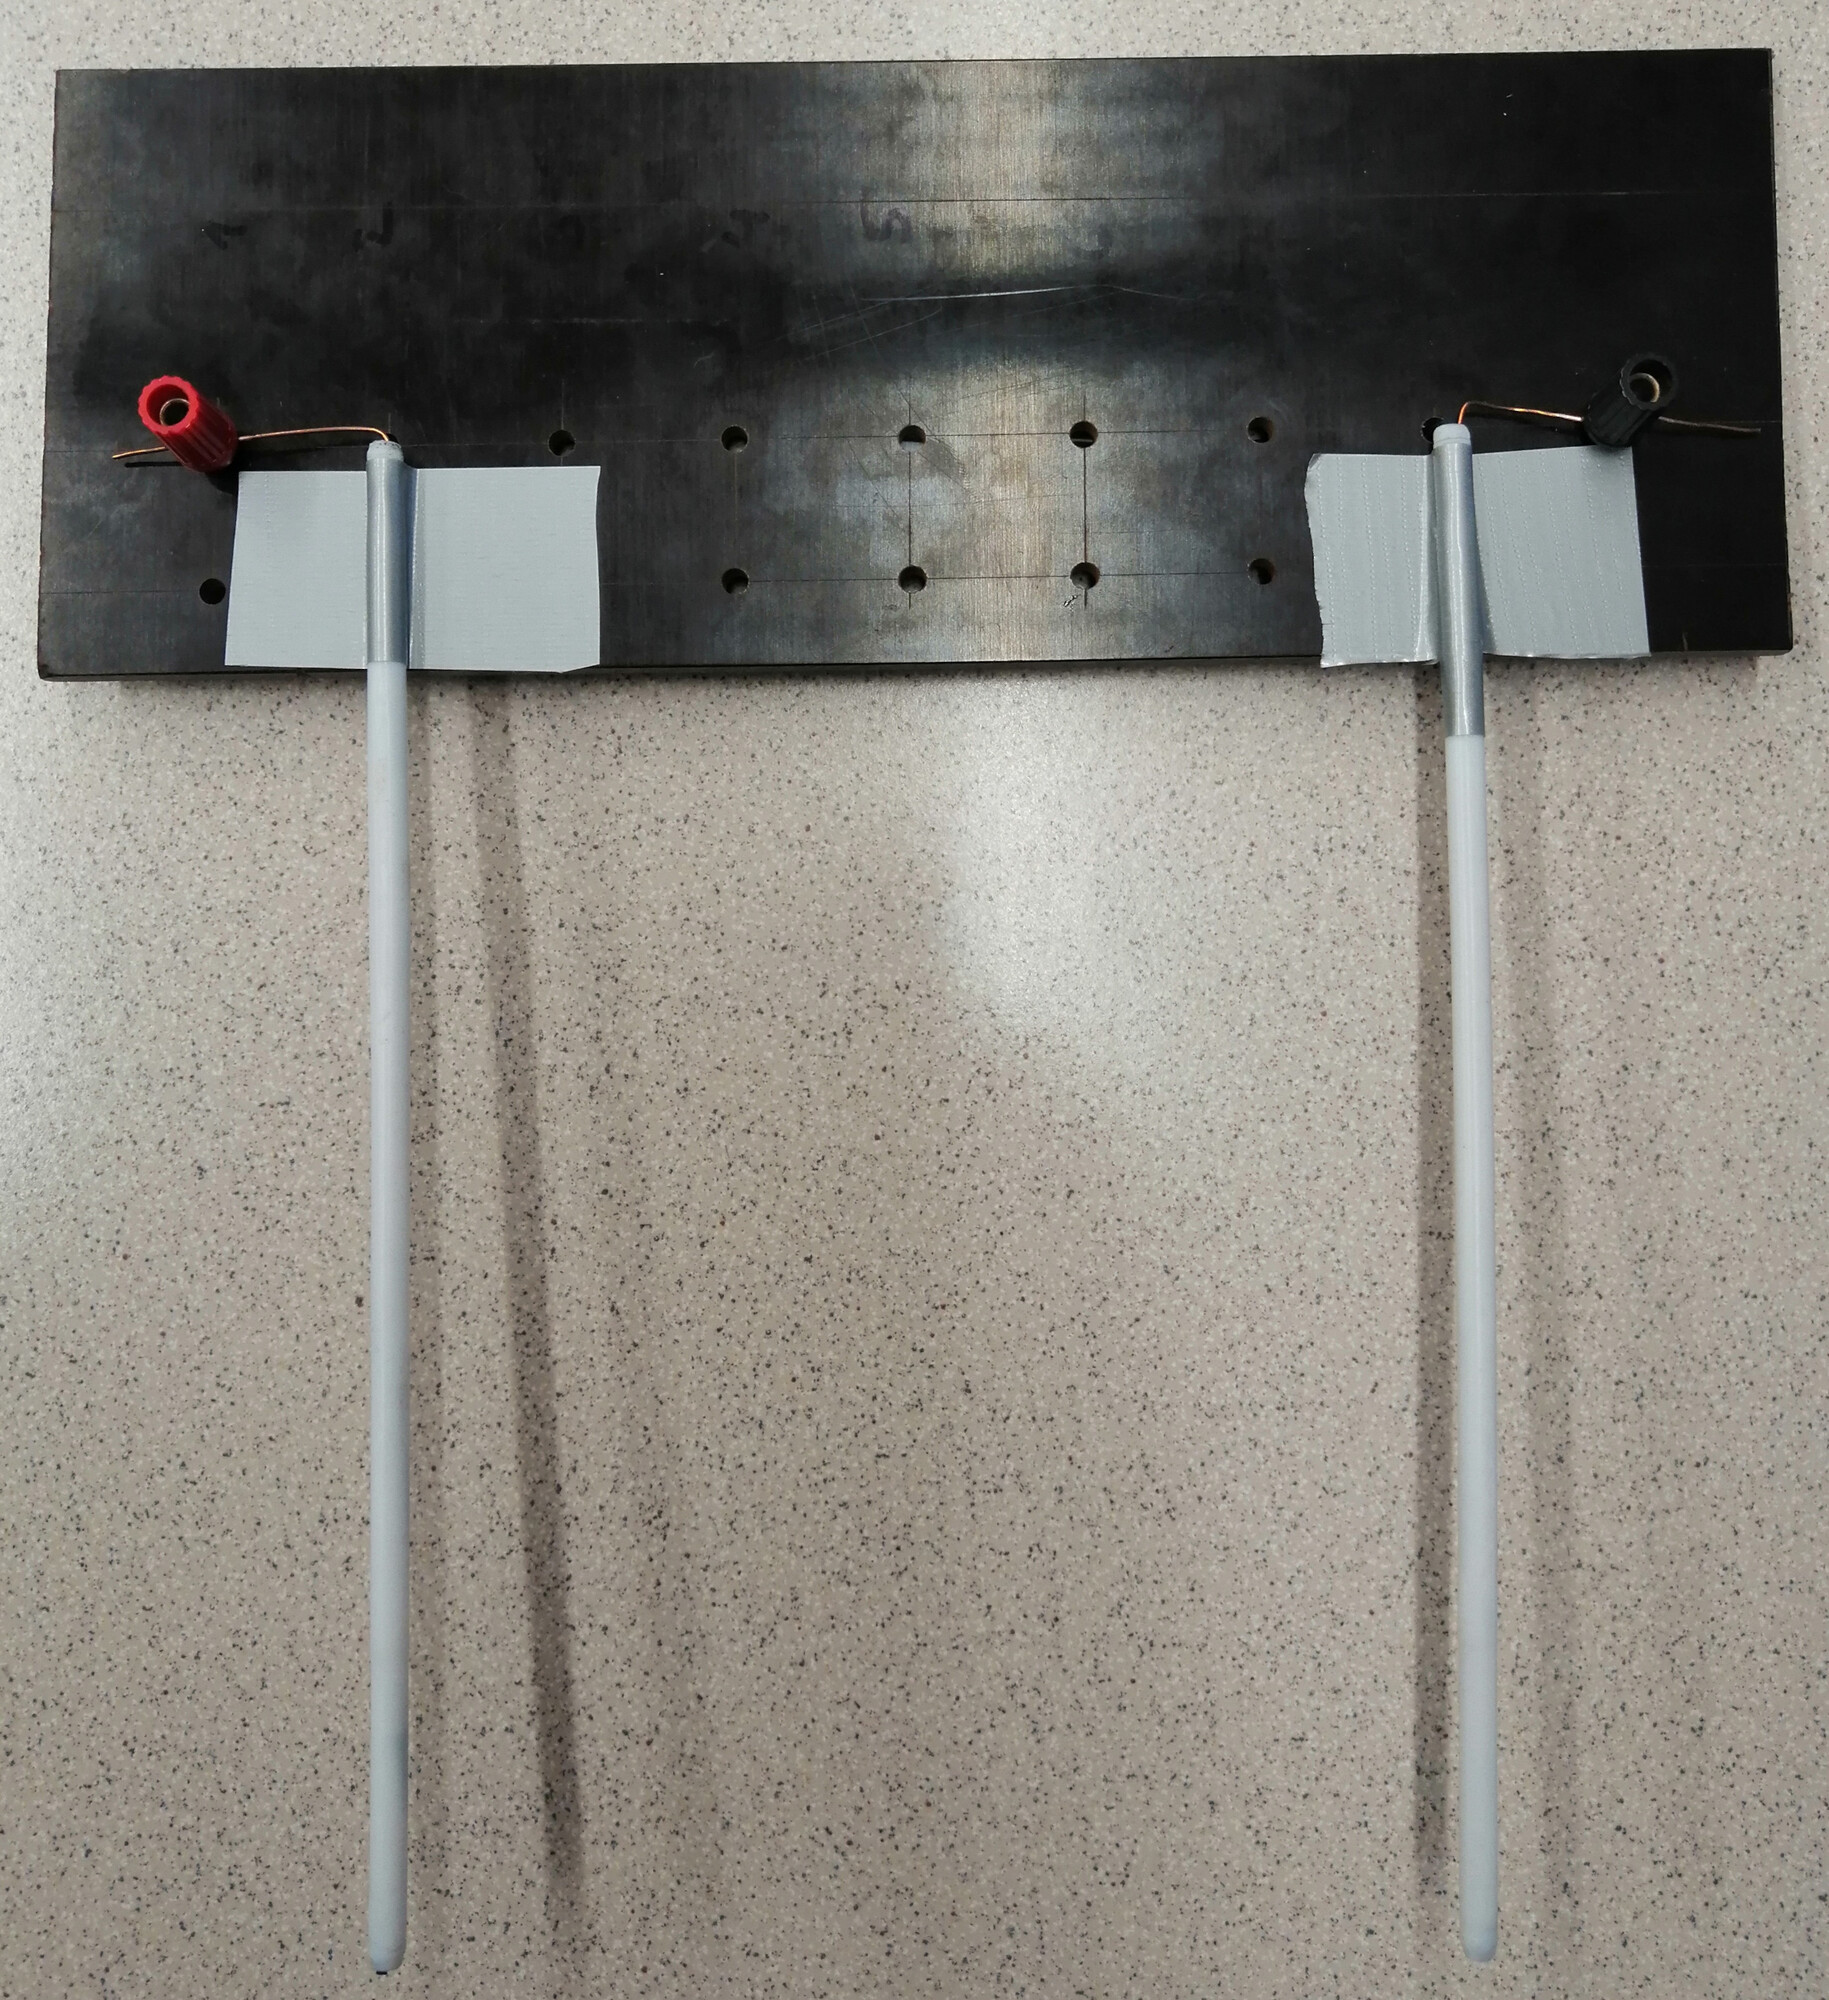
\includegraphics[height=0.8\textheight]{termoclanek_front.jpg}
			\caption{Přední strana}
		\end{subfigure}
		\hfill
		\begin{subfigure}{0.48\textwidth}
			\centering
			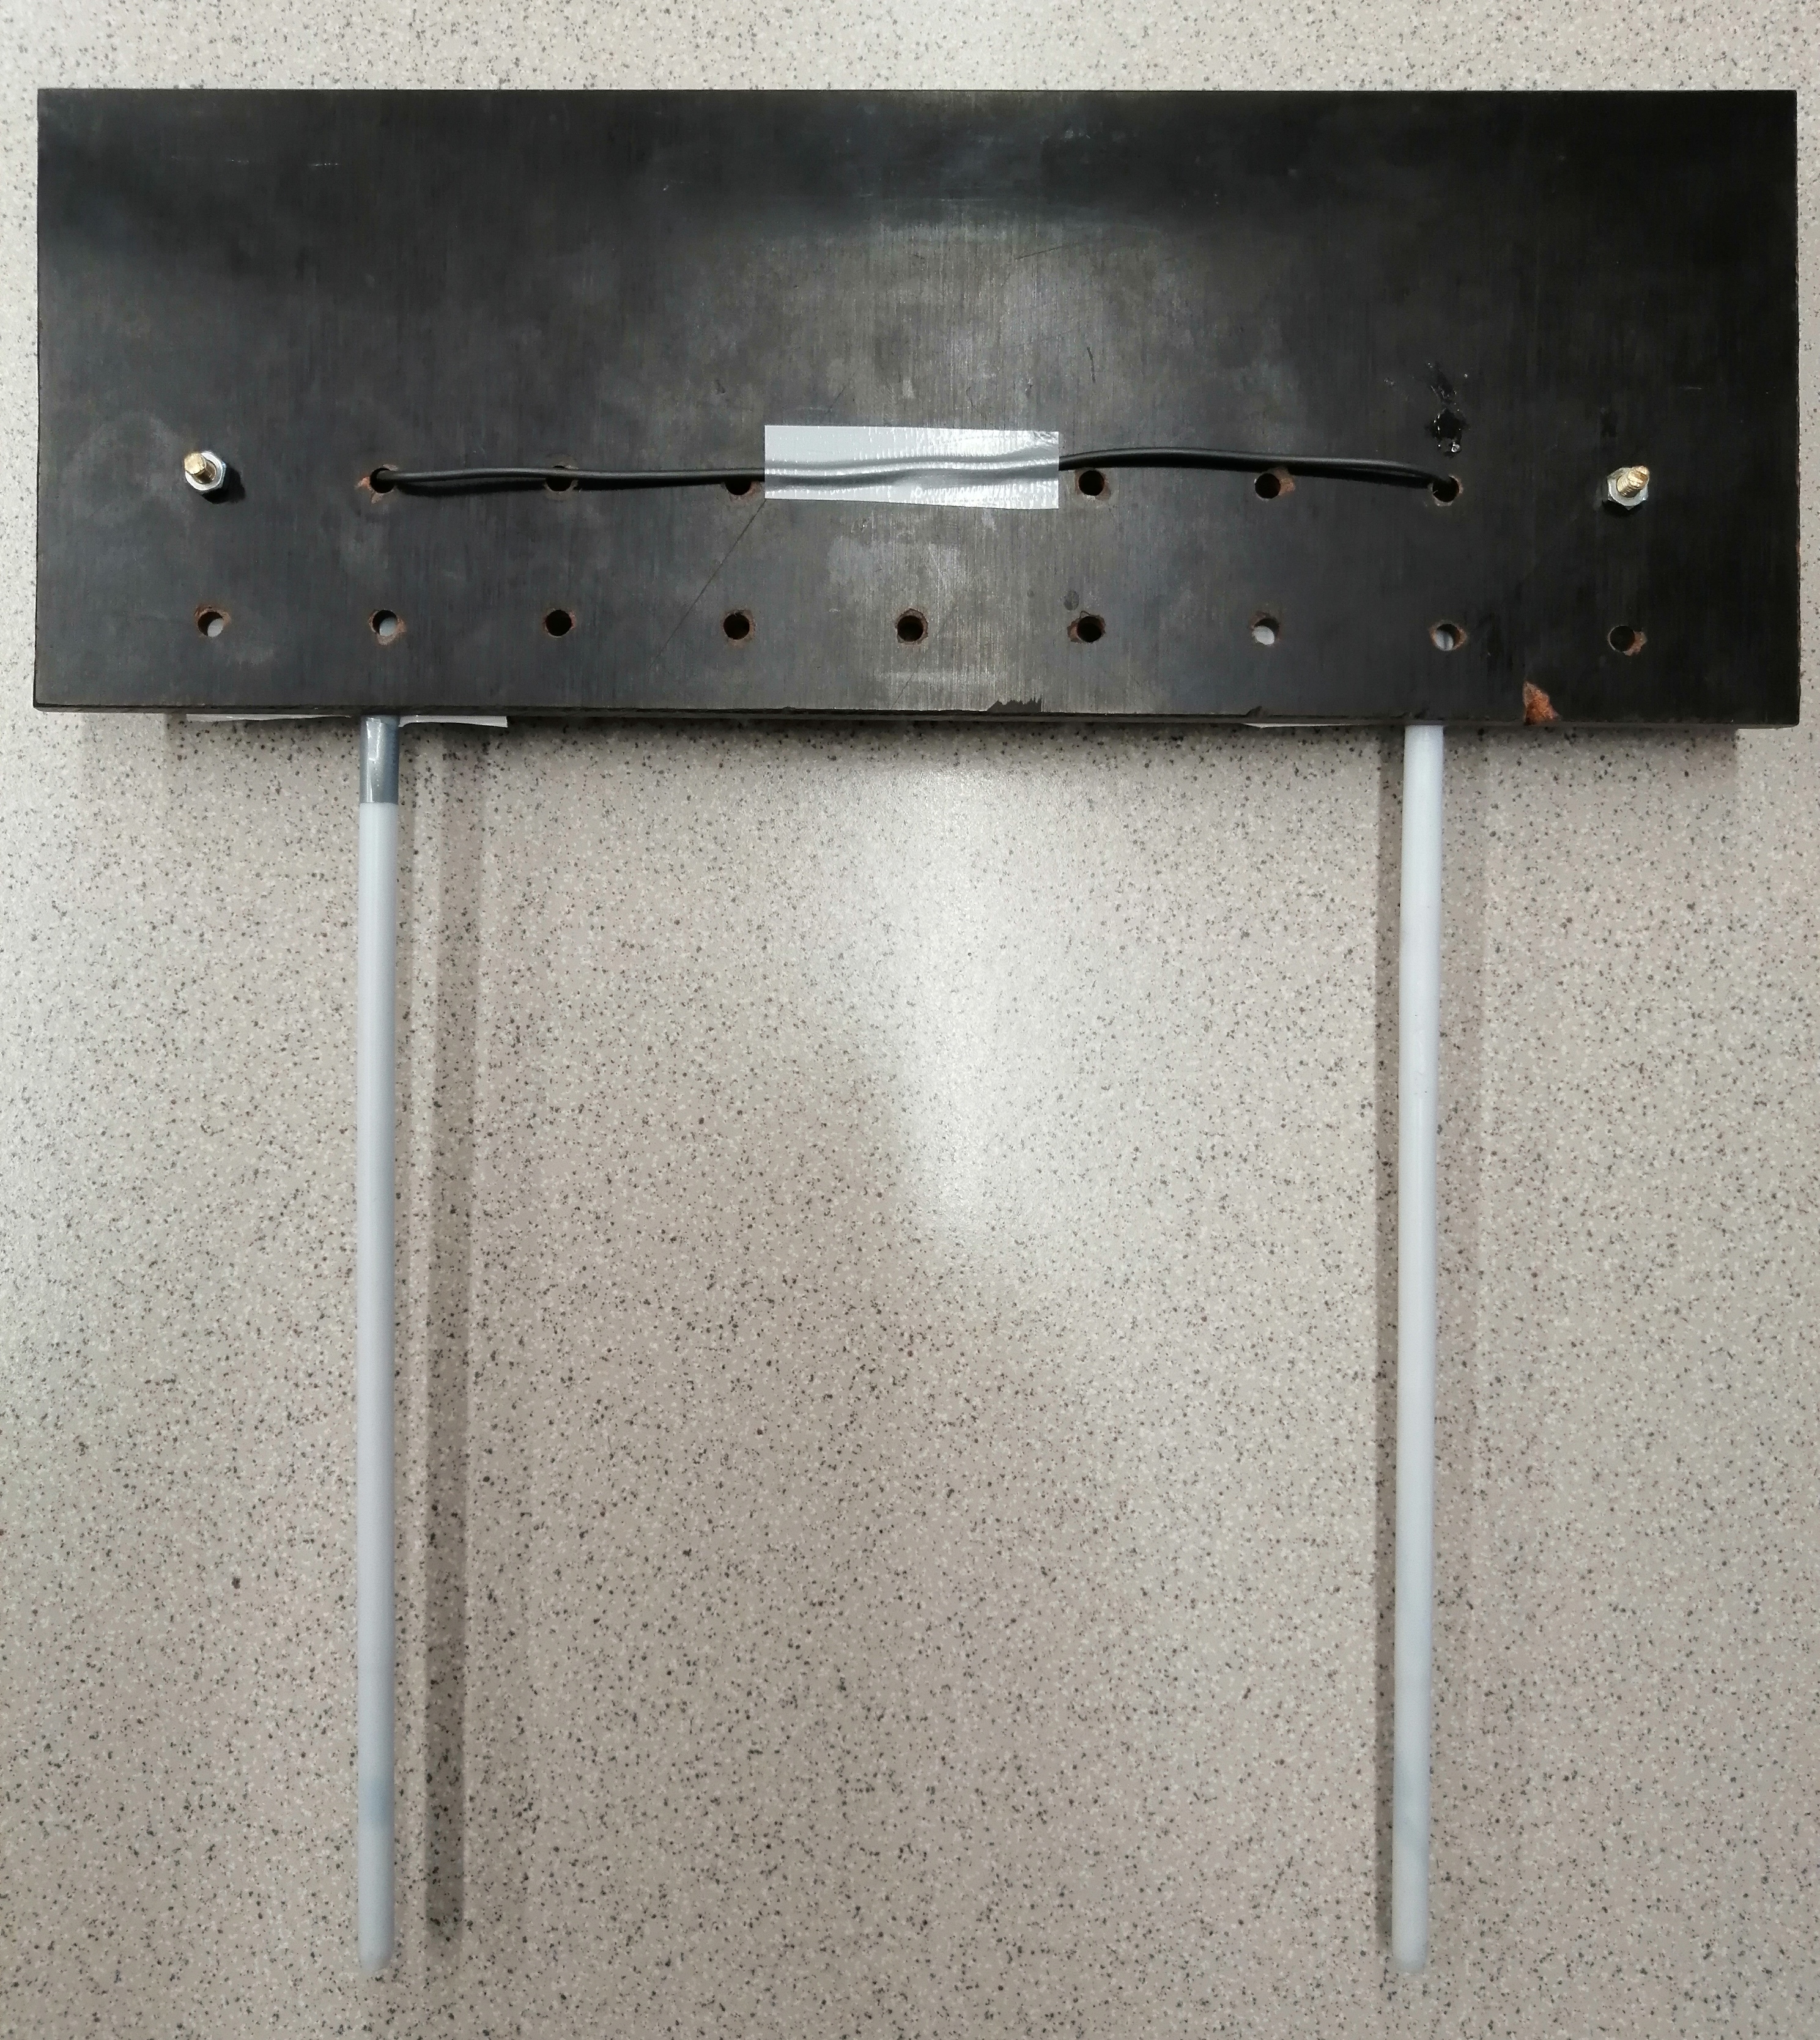
\includegraphics[height=0.8\textheight]{termoclanek_back.jpg}
			\caption{Zadní strana}
		\end{subfigure}
		\hfill
		\caption{Sestavený termočlánek}
		\label{fig:termoclanek}
	\end{figure}
\end{frame}

\begin{frame}
	\fullfig[width=0.9\textwidth][p]{aparatura.jpg}[Aparatura experimentu]
\end{frame}

\section{Výsledky}

\begin{frame}
	\frametitle{Výsledky}
	\framesubtitle{Tabulka dat}
	\hspace{0cm}\vfill
	\footnotesize
	\begin{table}[htbp]
    \centering
    \begin{tabular}{r|cccc|cc}
        \toprule
        $i$ & \popi{\Delta T}{\C} & \popi{E_1}{mV} & \popi{E_2}{mV} & \popi{\avg{E}}{mV} &
        \popi{\(\Delta T\)^2}{\C^2} & \popi{\Delta T * \avg{E}}{mV\C}\\
        \midrule
        $"1"$  & $"80"$ & $"2,8"$ & $"2,8"$ & $"2,8"$ & $"6~400"$ & $"224,0"$ \\
        $"2"$  & $"75"$ & $"2,8"$ & $"2,6"$ & $"2,7"$ & $"5~625"$ & $"202,5"$ \\
        $"3"$  & $"70"$ & $"2,6"$ & $"2,4"$ & $"2,5"$ & $"4~900"$ & $"175,0"$ \\
        $"4"$  & $"65"$ & $"2,4"$ & $"2,2"$ & $"2,3"$ & $"4~225"$ & $"149,5"$ \\
        $"5"$  & $"60"$ & $"2,2"$ & $"2,0"$ & $"2,1"$ & $"3~600"$ & $"126,0"$ \\
        $"6"$  & $"55"$ & $"2,0"$ & $"2,0"$ & $"2,0"$ & $"3~025"$ & $"110,0"$ \\
        $"7"$  & $"50"$ & $"1,8"$ & $"1,8"$ & $"1,8"$ & $"2~500"$ & $"90,0"$  \\
        $"8"$  & $"45"$ & $"1,8"$ & $"1,6"$ & $"1,7"$ & $"2~025"$ & $"76,5"$  \\
        $"9"$  & $"40"$ & $"1,6"$ & $"1,4"$ & $"1,5"$ & $"1~600"$ & $"60,0"$  \\
        $"10"$ & $"35"$ & $"1,2"$ & $"1,4"$ & $"1,3"$ & $"1~225"$ & $"45,5"$  \\
        $"11"$ & $"30"$ & $"1,2"$ & $"1,2"$ & $"1,2"$ & $"\phantom{0 }900"$   & $"36,0"$  \\
        $"12"$ & $"25"$ & $"1,0"$ & $"1,0"$ & $"1,0"$ & $"\phantom{0 }625"$   & $"25,0"$  \\
        $"13"$ & $"20"$ & $"1,0"$ & $"1,0"$ & $"1,0"$ & $"\phantom{0 }400"$   & $"20,0"$  \\
        \midrule
        \multicolumn{5}{r|}{$\sum$} & $"37~050"$ & $"1~340.0"$\\
        \bottomrule
    \end{tabular}
    \caption{Naměřená data}
    \label{tab:data}
\end{table}

	\vfill
\end{frame}

\begin{frame}
	\frametitle{Výsledky}
	\framesubtitle{Výpočet parametru}
	\begin{block}{Aproximace závislosti termoelektrického napětí při nízkém rozdílu teplot.}
		\centering $E=\alpha\Delta T$
	\end{block}
	\begin{block}{Výpočet parametru}
		\centering $a=\frac{\sumi x_iy_i}{\sumi x_i^2}
		\ztoho \alpha=\frac{\sumi\Delta T_i*E_i}{\sumi (\Delta T_i)^2}$
	\end{block}
\end{frame}

\begin{frame}
	\frametitle{Výsledky}
	\framesubtitle{Data v grafu}
	\hspace{0cm}\vfill
	\small
	\plotfig{graf/data-pres.tex}
	\vfill
\end{frame}

\begin{frame}
	\frametitle{Výsledky}
	\framesubtitle{Vypočtené parametry}
	\begin{columns}
		\begin{column}{0.46\textwidth}
			\begin{block}{Vypočtený parametr termočlánku}
				\centering $\alpha = "0.036~2 mV.C^{-1}"$
			\end{block}
		\end{column}
		\begin{column}{0.46\textwidth}
			\begin{block}{Tabulková hodnota parametru}
				\centering $\alpha = "0.042 \micro V.C^{-1}"$
			\end{block}
		\end{column}
	\end{columns}
	\begin{block}{Rozptyl naměřených dat}
		\centering $R^2="0.958~5"="95.85 \%"$
	\end{block}
\end{frame}

\section{Diskuze}
\begin{frame}
	\frametitle{Diskuze}
	\begin{itemize}
		\item odlišná vypočtená a tabulková hodnota, malý rozptyl 
			hodnot~$\rightarrow$ systémová chyba
		\item provedení experimentu vícekrát
		\item použití digitálního voltmetru
		\item provedení experimentu při zahřívání i ochlazování
	\end{itemize}
\end{frame}

\section{Závěr}
\begin{frame}
	\frametitle{Závěr}
	\begin{itemize}
		\item metoda nejmenších čtverců je důležitá v prokládání dat funkcí
		\item termočlánek -- dva spolu spojené druhy kovů, na kterých se
			projevuje termoelektrický jev
		\item nutno měřit koeficienty pro každou dvojici kovů
		\item termočlánek typu T
			\begin{itemize}
				\item tabulková hodnota: $\alpha = "0.036~2 mV.C^{-1}"$
				\item experimentální hodnota: $\alpha = "0.042 mV.C^{-1}"$
			\end{itemize}
		\item přesnost našeho měření: $R^2="0.958~5"="95.85 \%"$
	\end{itemize}
\end{frame}

%\begin{frame}[allowframebreaks=.85]{Zdroje}
%	\setbeamertemplate{bibliography item}{}
%	\nocite{*}
%    \printbibliography[heading=none]
%\end{frame}

\part{}

\begin{frame}[plain]
	\titlepage
\end{frame}
\end{document}
